\section{Introducción}

Este manual describe el uso del Sistema de Exámenes de Colocación del Centro Boliviano Americano (CBA), tanto para estudiantes como para administradores.

\section{Módulo Estudiante}

\subsection{Registro}

El estudiante debe registrarse en el sistema proporcionando los siguientes datos:

\begin{itemize}
    \item Carnet de Identidad (CI)
    \item Nombre completo
    \item Correo electrónico
    \item Contraseña
    \item Teléfono (opcional)
\end{itemize}

\begin{figure}[H]
\centering
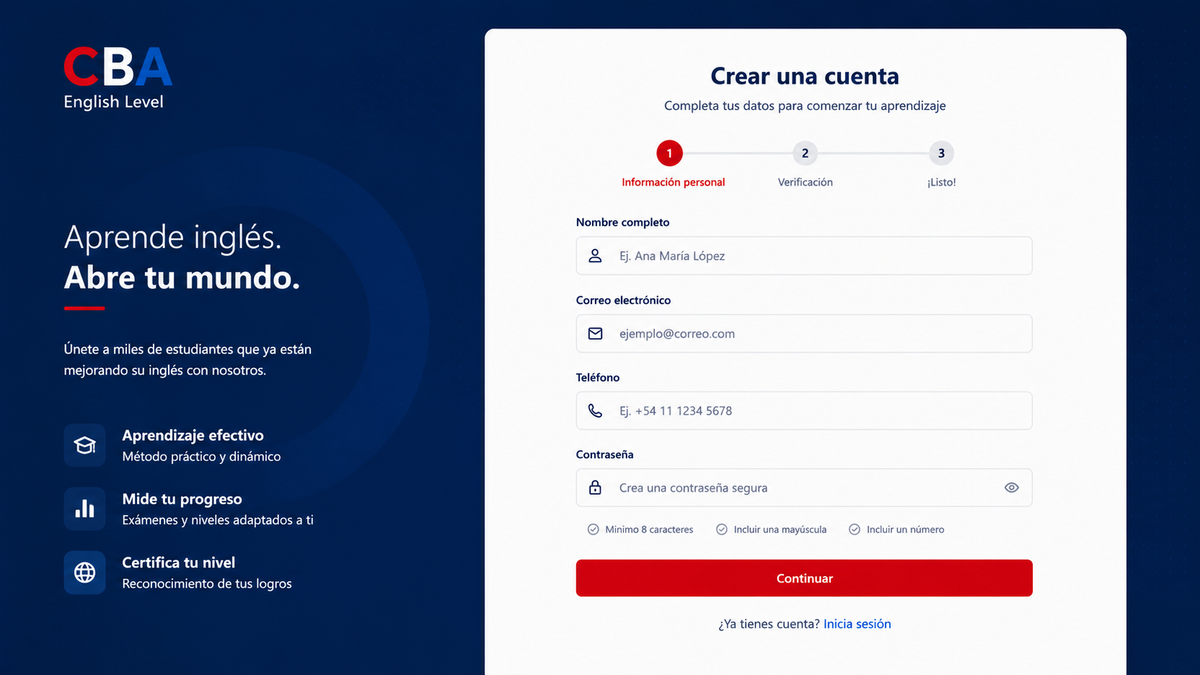
\includegraphics[width=0.7\textwidth]{imagenes/registro.png}
\caption{Pantalla de registro de estudiante}
\end{figure}

\subsection{Inicio de Sesión}

El estudiante puede iniciar sesión ingresando su CI o correo electrónico junto con su contraseña.

\begin{figure}[H]
\centering
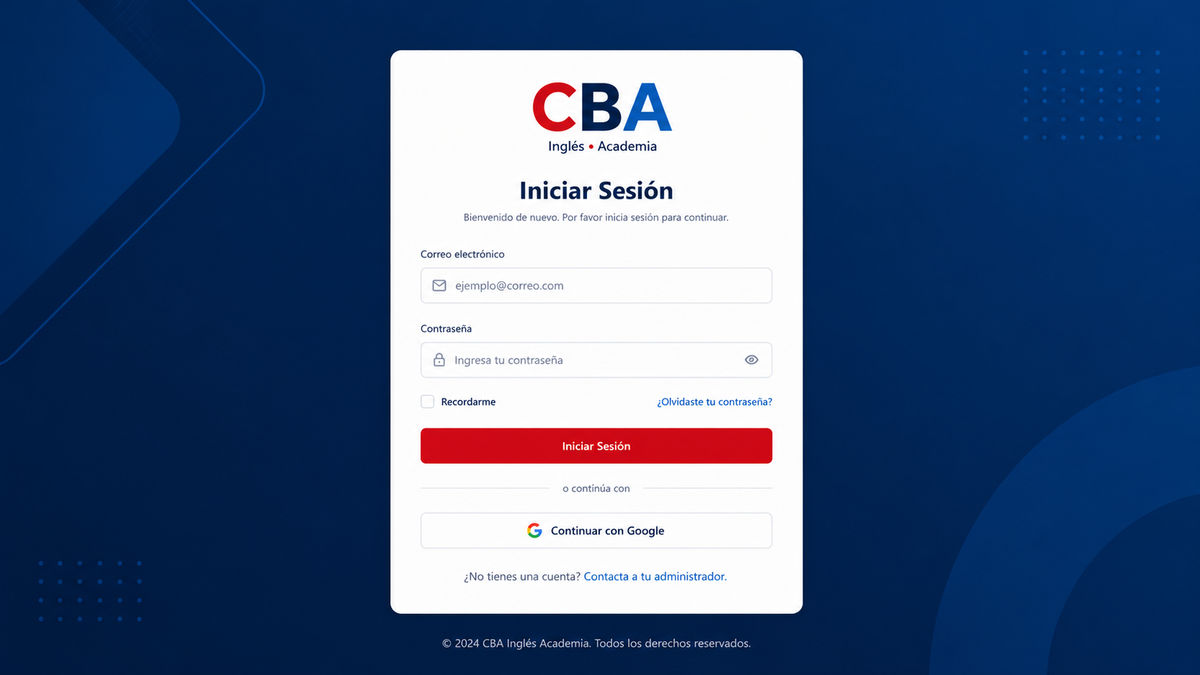
\includegraphics[width=0.7\textwidth]{imagenes/login.png}
\caption{Pantalla de inicio de sesión}
\end{figure}

\subsection{Rendir Examen}

Una vez autenticado, el estudiante puede solicitar un nuevo examen. El sistema presenta las preguntas de forma aleatoria con un temporizador visible. Al agotarse el tiempo, el examen se envía automáticamente.

\begin{figure}[H]
\centering
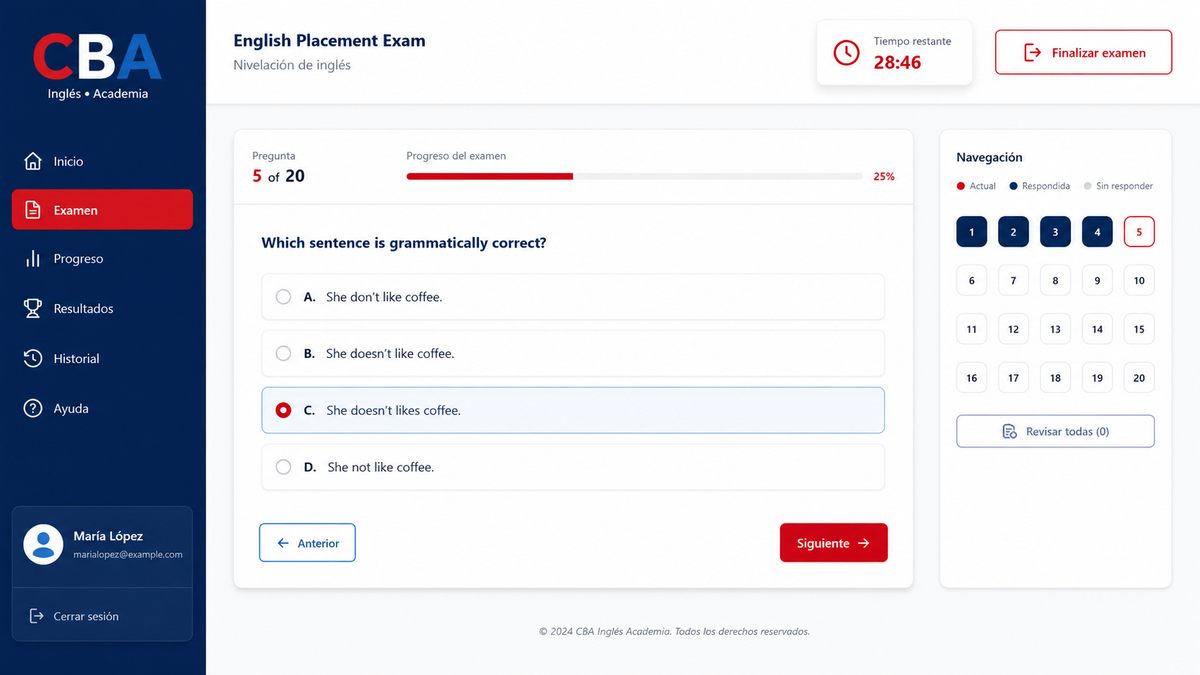
\includegraphics[width=0.7\textwidth]{imagenes/mockup.png}
\caption{Pantalla principal del examen}
\end{figure}

\subsection{Resultado}

Al finalizar el examen, el sistema muestra el puntaje obtenido y el nivel de inglés asignado de forma inmediata.

\begin{figure}[H]
\centering
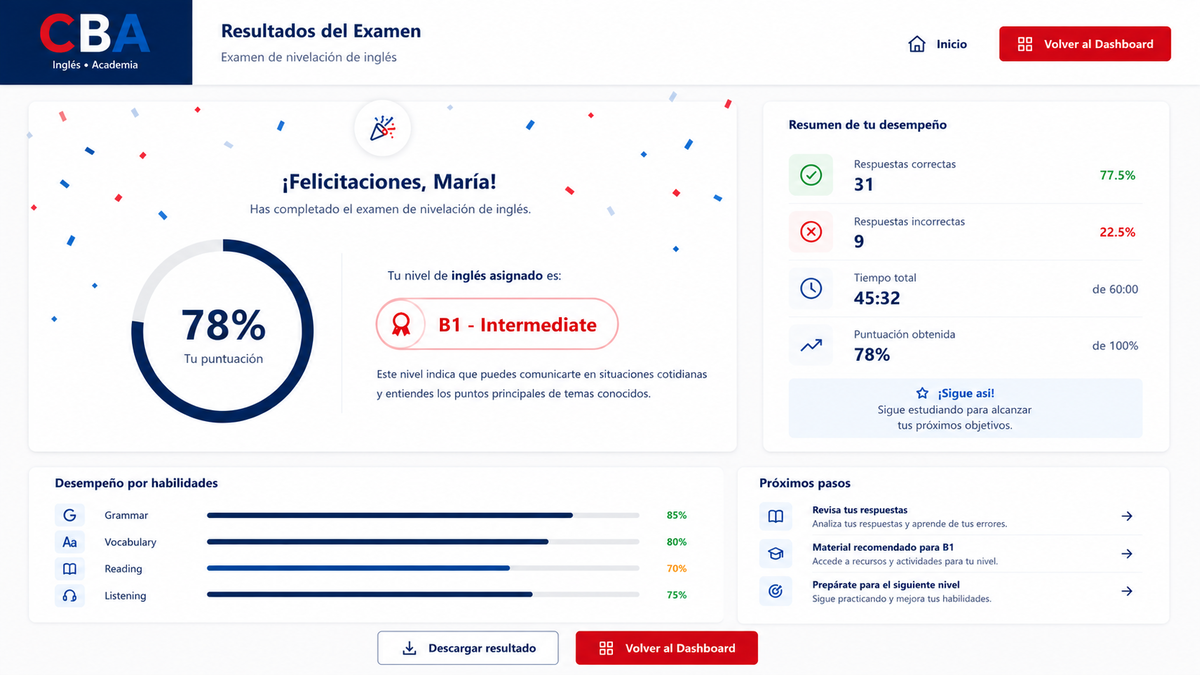
\includegraphics[width=0.7\textwidth]{imagenes/resultado.png}
\caption{Pantalla de resultado del examen}
\end{figure}

\section{Módulo Administrador}

\subsection{Acceso}

El administrador accede al panel de administración mediante un inicio de sesión seguro con su correo electrónico y contraseña.

\subsection{Dashboard}

El dashboard principal muestra estadísticas generales del sistema: cantidad de estudiantes registrados, exámenes rendidos, distribución de niveles y actividad reciente.

\begin{figure}[H]
\centering
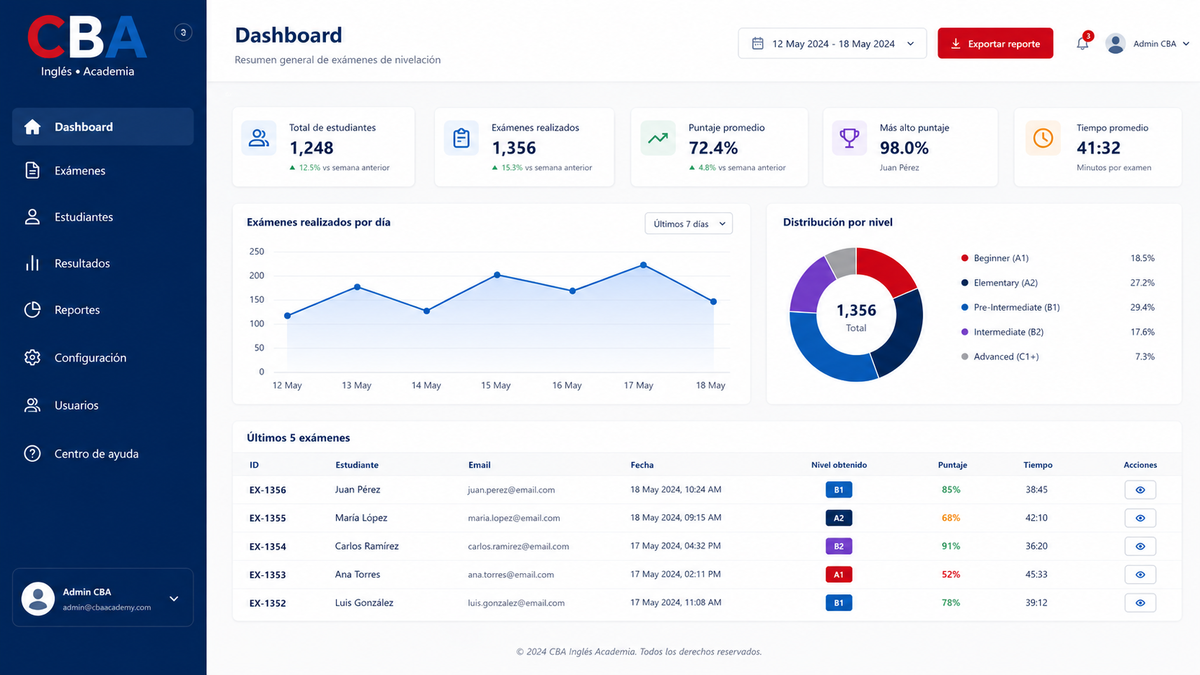
\includegraphics[width=0.7\textwidth]{imagenes/dashboard.png}
\caption{Dashboard administrativo}
\end{figure}

\subsection{Gestión de Preguntas}

El administrador puede crear, editar y eliminar preguntas. Cada pregunta incluye:

\begin{itemize}
    \item Enunciado de la pregunta.
    \item Cuatro opciones de respuesta (con una correcta).
    \item Nivel de inglés asociado.
    \item Categoría opcional (grammar, vocabulary, reading).
\end{itemize}

\subsection{Gestión de Niveles}

El administrador puede configurar los niveles de inglés, definiendo para cada uno:

\begin{itemize}
    \item Nombre del nivel.
    \item Rango de puntaje (mínimo y máximo).
    \item Descripción opcional.
\end{itemize}

\subsection{Configuración del Examen}

El administrador puede modificar los parámetros globales del examen:

\begin{itemize}
    \item Tiempo límite en minutos.
    \item Cantidad de preguntas por examen.
    \item Puntaje mínimo de aprobación.
\end{itemize}

\subsection{Reportes}

El sistema permite exportar reportes en los siguientes formatos:

\begin{itemize}
    \item \textbf{CSV}: Datos de estudiantes, exámenes y resultados.
    \item \textbf{Excel}: Reportes detallados con formato profesional.
\end{itemize}

Los reportes incluyen:

\begin{itemize}
    \item Listado de estudiantes registrados.
    \item Historial de exámenes por estudiante.
    \item Distribución de niveles alcanzados.
    \item Estadísticas de aprobación por período.
\end{itemize}
